\documentclass{standalone}
\usepackage{graphicx}	
\usepackage{amssymb, amsmath}
\usepackage{color}

\usepackage{tikz}
\usetikzlibrary{intersections, backgrounds, math}
\usepackage{pgfmath}

\definecolor{light}{RGB}{220, 188, 188}
\definecolor{mid}{RGB}{185, 124, 124}
\definecolor{dark}{RGB}{143, 39, 39}
\definecolor{darker}{RGB}{124, 0, 0}
\definecolor{highlight}{RGB}{180, 31, 180}
\definecolor{light_teal}{RGB}{107, 142, 142}
\definecolor{mid_teal}{RGB}{72, 117, 117}
\definecolor{dark_teal}{RGB}{29, 79, 79}
\definecolor{gray10}{gray}{0.1}
\definecolor{gray20}{gray}{0.2}
\definecolor{gray30}{gray}{0.3}
\definecolor{gray40}{gray}{0.4}
\definecolor{gray60}{gray}{0.6}
\definecolor{gray70}{gray}{0.7}
\definecolor{gray80}{gray}{0.8}
\definecolor{gray90}{gray}{0.9}
\definecolor{gray95}{gray}{0.95}

\begin{document}

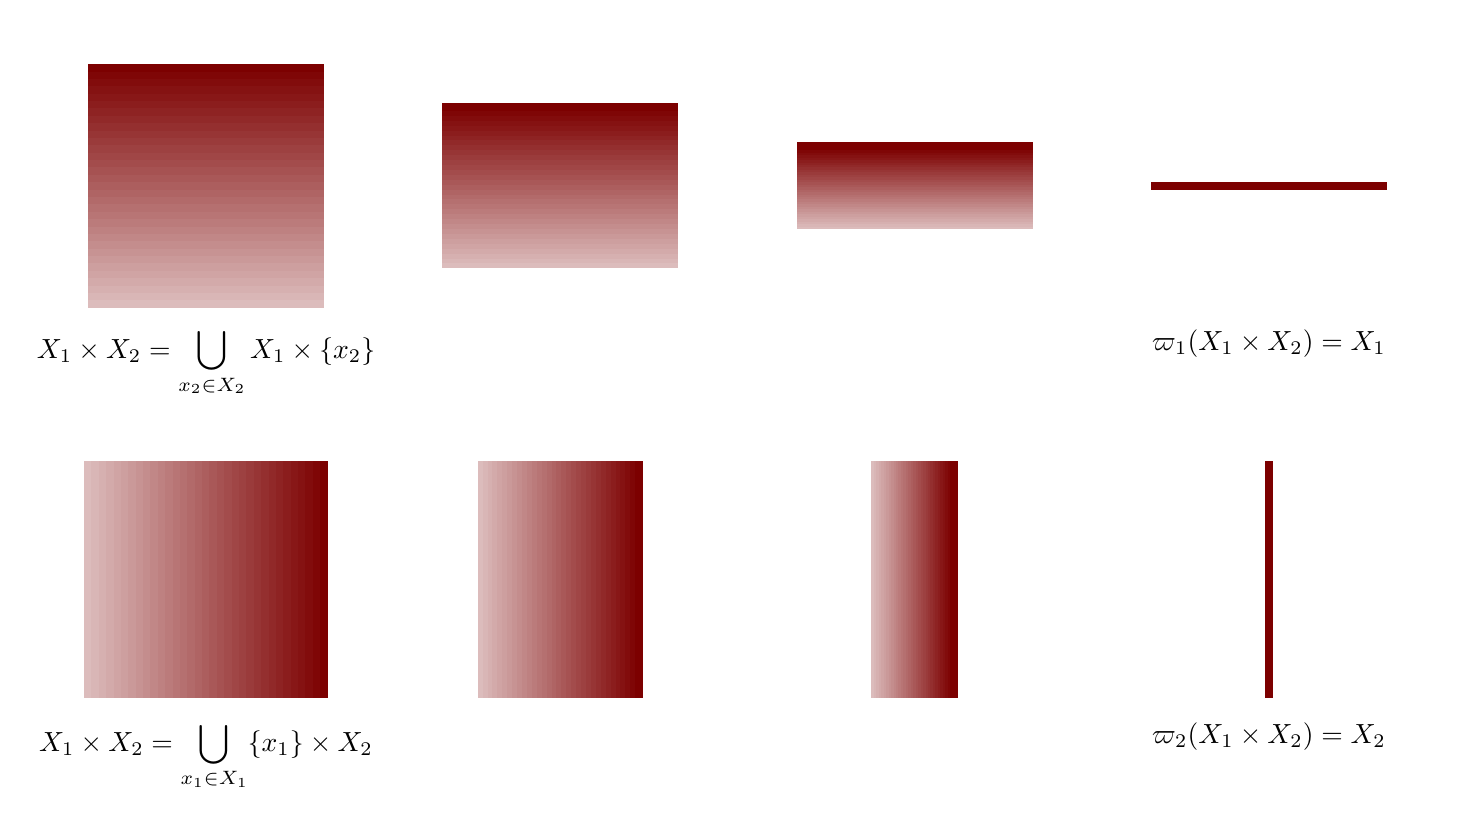
\begin{tikzpicture}[scale=1.0]
 
  \pgfmathsetmacro{\delta}{1.6 / 32}

  \begin{scope}[shift={(0, -5)}]
    \draw[white] (-2.25, -2.75) rectangle (2.25, 2);
    
    \foreach \n in {0, 1, ..., 32} {
      \pgfmathsetmacro{\xi}{1.5 * (\n / 16 - 1)}
      \pgfmathsetmacro{\prop}{100 * \n / 32}
      \colorlet{custom}{darker!\prop!light};
      \fill[custom]    (\xi - \delta, -1.5) -- (\xi + \delta, -1.5) 
                    -- (\xi + \delta, +1.5) -- (\xi - \delta, +1.5) -- cycle;
    }
        
    \node at (0, -2.25)
      { $X_{1} \times X_{2} = \displaystyle \bigcup_{x_{1} \in X_{1}} \{ x_{1}  \} \times X_{2}$ };
  \end{scope}

  \begin{scope}[shift={(4.5, -5)}]
    \draw[white] (-2.25, -2.75) rectangle (2.25, 2);
    
    \foreach \n in {0, 1, ..., 32} {
      \pgfmathsetmacro{\xi}{1.0 * (\n / 16 - 1)}
      \pgfmathsetmacro{\prop}{100 * \n / 32}
      \colorlet{custom}{darker!\prop!light};
      \fill[custom]    (\xi - \delta, -1.5) -- (\xi + \delta, -1.5) 
                    -- (\xi + \delta, +1.5) -- (\xi - \delta, +1.5) -- cycle;
    }
  \end{scope}
  
  \begin{scope}[shift={(9.0, -5)}]
    \draw[white] (-2.25, -2.75) rectangle (2.25, 2);
    
    \foreach \n in {0, 1, ..., 32} {
      \pgfmathsetmacro{\xi}{0.5 * (\n / 16 - 1)}
      \pgfmathsetmacro{\prop}{100 * \n / 32}
      \colorlet{custom}{darker!\prop!light};
      \fill[custom]    (\xi - \delta, -1.5) -- (\xi + \delta, -1.5) 
                    -- (\xi + \delta, +1.5) -- (\xi - \delta, +1.5) -- cycle;
    }
  \end{scope}
  
  \begin{scope}[shift={(13.5, -5)}]
    \draw[white] (-2.25, -2.75) rectangle (2.25, 2);
    
    \foreach \n in {0, 1, ..., 32} {
      \pgfmathsetmacro{\xi}{0.0 * (\n / 16 - 1)}
      \pgfmathsetmacro{\prop}{100 * \n / 32}
      \colorlet{custom}{darker!\prop!light};
      \fill[custom]    (\xi - \delta, -1.5) -- (\xi + \delta, -1.5) 
                    -- (\xi + \delta, +1.5) -- (\xi - \delta, +1.5) -- cycle;
    }
        
    \node at (0, -2) { $\varpi_{2}(X_{1} \times X_{2}) = X_{2}$ };
  \end{scope}

  \begin{scope}[shift={(0, 0)}]
    \draw[white] (-2.25, -2.75) rectangle (2.25, 2);
    
    \foreach \n in {0, 1, ..., 32} {
      \pgfmathsetmacro{\eta}{1.5 * (\n / 16 - 1) + 0}
      \pgfmathsetmacro{\prop}{100 * \n / 32}
      \colorlet{custom}{darker!\prop!light}; 
      \fill[custom]    (-1.5, \eta - \delta) -- (-1.5, \eta + \delta) 
                    -- (+1.5, \eta + \delta) -- (+1.5, \eta - \delta);
    }
        
    \node at (0, -2.25) 
      { $X_{1} \times X_{2} = \displaystyle \bigcup_{x_{2} \in X_{2}} X_{1} \times \{ x_{2} \}$ };
  \end{scope}

  \begin{scope}[shift={(4.5, 0)}]
    \draw[white] (-2.25, -2.75) rectangle (2.25, 2);
    
    \foreach \n in {0, 1, ..., 32} {
      \pgfmathsetmacro{\eta}{1.0 * (\n / 16 - 1) + 0}
      \pgfmathsetmacro{\prop}{100 * \n / 32}
      \colorlet{custom}{darker!\prop!light}; 
      \fill[custom]    (-1.5, \eta - \delta) -- (-1.5, \eta + \delta) 
                    -- (+1.5, \eta + \delta) -- (+1.5, \eta - \delta);
    }
  \end{scope}
  
  \begin{scope}[shift={(9, 0)}]
    \draw[white] (-2.25, -2.75) rectangle (2.25, 2);
    
    \foreach \n in {0, 1, ..., 32} {
      \pgfmathsetmacro{\eta}{0.5 * (\n / 16 - 1) + 0}
      \pgfmathsetmacro{\prop}{100 * \n / 32}
      \colorlet{custom}{darker!\prop!light}; 
      \fill[custom]    (-1.5, \eta - \delta) -- (-1.5, \eta + \delta) 
                    -- (+1.5, \eta + \delta) -- (+1.5, \eta - \delta);
    }
  \end{scope}
  
  \begin{scope}[shift={(13.5, 0)}]
    \draw[white] (-2.25, -2.75) rectangle (2.25, 2);
    
    \foreach \n in {0, 1, ..., 32} {
      \pgfmathsetmacro{\eta}{0.0 * (\n / 16 - 1) + 0}
      \pgfmathsetmacro{\prop}{100 * \n / 32}
      \colorlet{custom}{darker!\prop!light}; 
      \fill[custom]    (-1.5, \eta - \delta) -- (-1.5, \eta + \delta) 
                    -- (+1.5, \eta + \delta) -- (+1.5, \eta - \delta);
    }
        
    \node at (0, -2) { $\varpi_{1}(X_{1} \times X_{2}) = X_{1}$ };
  \end{scope}

\end{tikzpicture}

\end{document}  